\documentclass[border=3pt,tikz]{standalone}
\usepackage{minkowski}

\begin{document}
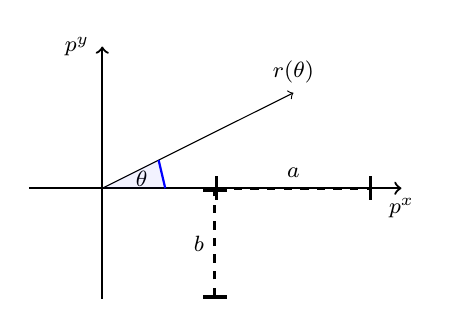
\begin{tikzpicture}[scale=2.0]
    \def\xrange{1.4}

    \coordinate (O) at (0,0);
    \coordinate (T) at (0,\xrange+0.2);
    \coordinate (A) at (1.2, 1.2);
    \coordinate (B) at (-0.8, 0.8);
    \coordinate (C) at (0, 0.96);

    \draw[->,thick] (0,-\xrange/2) -- (0,\xrange/2+0.2) node[left=1] {\footnotesize $p^y$};
    \draw[->,thick] (-\xrange/3,0) -- (\xrange+0.5,0) node[below=0] {\footnotesize $p^x$};

    \def\a{1}
    \def\b{0.7}

    \draw[black,samples=\Nsamples,smooth,variable=\x,domain=0:360] plot({sqrt(\a*\a - \b*\b) + (\a * cos(\x))},{(\b * sin(\x))});

    \draw[black,->] (O) -- ({sqrt(\a*\a - \b*\b) + (\a * cos(60))},{\b * sin(60)}) node[above] {\footnotesize $r(\theta)$};
    \draw[blue,thick,samples=\Nsamples,smooth,variable=\x,domain=0:26.5] plot({0.4*cos(\x))},{(0.4*sin(\x))}) node[text=black] at (0.25,0.06) {\footnotesize $\theta$};
    \fill[blue,opacity=0.05,thick,samples=\Nsamples,smooth,variable=\x,domain=0:26.5]
        plot({0.4*cos(\x))},{(0.4*sin(\x))}) -- (O);

    \draw[black,|-|,dashed,very thick] ({\a+sqrt(\a*\a - \b*\b)-\a},0) -- ({sqrt(\a*\a - \b*\b) + \a},0) node[midway,above] {\footnotesize $a$};

    \draw[black,|-|,dashed,very thick] ({sqrt(\a*\a - \b*\b)},-\b) -- ({sqrt(\a*\a - \b*\b)},0) node[midway,left] {\footnotesize $b$};

\end{tikzpicture}
\end{document}
